\documentclass{article}
\usepackage{template}

\usepackage{chngcntr} % Reset counter within sections
\usepackage{circuitikz}

\counterwithin*{equation}{section}
\counterwithin*{equation}{subsection}

\pagestyle{fancy}
\setlength\headheight{24pt}

\lhead{\className}
\rhead{\leftmark}
\cfoot{\thepage}

\newcommand{\uniTitle}{Queensland University of Technology}
\newcommand{\className}{Foundations of Electrical Engineering}
\newcommand{\classTime}{Semester 2, 2021}
\newcommand{\classInstructorName}{Dr Jasmin Martin}
\newcommand{\authorName}{Tarang Janawalkar}
\newcommand{\authorStudentNumber}{n11032201}
\newcommand{\classCode}{EGB120}

\usepackage[
    type={CC},
    modifier={by-nc-sa},
    version={4.0},
    imagewidth={5em},
]{doclicense}

\date{}

\begin{document}
\begin{titlepage}
    \vspace*{\fill}
	\begin{center}
        \LARGE
        \textbf{\className}
        \texorpdfstring{\\}{ }
        \uniTitle
        \texorpdfstring{\\}{ }
        \texorpdfstring{\vspace{0.3in}}{ }
        \normalsize\textit{\classInstructorName}
        \texorpdfstring{\\}{ }
        \classTime
    \end{center}
    \begin{center}
        \textbf{\authorName}
    \end{center}
    \vspace*{\fill}
    \doclicenseThis
    \thispagestyle{empty}
\end{titlepage}
\newpage

\tableofcontents
\newpage

\section{Electrical Circuits}
\subsection{Fundamental Quantities}
\begingroup
\renewcommand{\arraystretch}{1.5}
\begin{table}[H]
    \centering
    \begin{tabular}{c | >{\centering}p{0.5\textwidth} | c c}
        \toprule
        \textbf{Name} & \textbf{Definition} & \textbf{Symbol} & \textbf{Unit} \\
        \midrule
        Charge & Electric charge is a fundamental property of matter that governs how particles are affected by an electromagnetic field.
        & $q$ & Coulomb (\unit{\coulomb}) \\
        \hline
        Current & $i=\dv{q}{t}\iff\SI{1}{\ampere}=\SI{1}{\coulomb\per\s}$
        & $i$ & Ampere (\unit{\ampere}) \\
        \hline
        Voltage & $v=\dv{w}{q}\iff\SI{1}{\volt}=\SI{1}{\joule\per\coulomb}$
        & $v$ & Volt (\unit{\volt}) \\
        \hline
        Power & $p=\dv{w}{t}\iff\SI{1}{\watt}=\SI{1}{\joule\per\s}$
        & $p$ & Watt (\unit{\watt}) \\
        \bottomrule
    \end{tabular}
\end{table}
\endgroup
\begin{description}
    \item[Charge in an electron.] $q=\SI{1.6022e-19}{\coulomb}$.
    \item[Electric Power.] $p=\dv{w}{t}=\frac{\dd{w}}{\cancel{\dd{q}}} \frac{\cancel{\dd{q}}}{\dd{t}}=vi$. 
\end{description}
\subsection{Passive Sign Convention}
\begin{figure}[H]
    \centering
    \begin{minipage}[H]{0.48\textwidth}
        \textbf{Passive component}
        \centering
        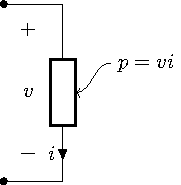
\includegraphics[height = 4cm, keepaspectratio = true]{passive_component}
        \caption{Energy dissipated.}
    \end{minipage}\hfill
    \begin{minipage}[H]{0.48\textwidth}
        \textbf{Active component}
        \centering
        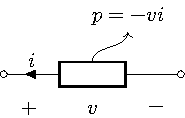
\includegraphics[height = 4cm, keepaspectratio = true]{active_component}
        \caption{Energy produced.}
    \end{minipage}
\end{figure}
\begin{theorem}[Power Balance]
    \begin{equation*}
        p_{\mathrm{net}} = 0
    \end{equation*}
\end{theorem}
\begin{theorem}[Energy]
    \begin{equation*}
        w\left( \tau \right) = \int_0^\tau p\left( t \right) \dd{t}
    \end{equation*}
\end{theorem}
\subsection{Circuits and Sources}
\begin{definition}[Circuits]
    A circuit is a mathematical model that approximates a real system. It is built from ideal circuit elements connected by ideal wires. 
\end{definition}
\begin{definition}[Voltage Source]
    Produces or dissipates power at a specified voltage with whatever current is required. 
\end{definition}
\begin{figure}[H]
    \centering
    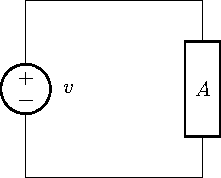
\includegraphics{voltage_source}
    \caption{Voltage Source -- $v$ is specified, $i$ varies depending on circuit element $A$.}
\end{figure}
\begin{definition}[Current Source]
    Produces or dissipates power at a specified current with whatever voltage is required. 
\end{definition}
\begin{figure}[H]
    \centering
    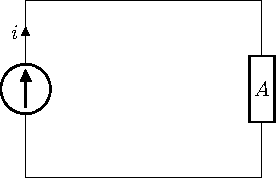
\includegraphics{current_source}
    \caption{Current Source -- $i$ is specified, $v$ varies depending on circuit element $A$.}
\end{figure}
\subsection{Ground}
\begin{description}
    \item[Definition.] The zero volt point is referred to as the circuit ground.
    \item[Symbol.] \tikz\draw (0, 0) node [sground] {};
\end{description}
\subsection{Earth}
\begin{description}
    \item[Definition.] An earthed ground is literally a connection to the earth.
    \item[Symbol.] \tikz\draw (0, 0) node [ground] {};
\end{description}
\subsection{Connected Sources}
\begin{figure}[H]
    \centering
    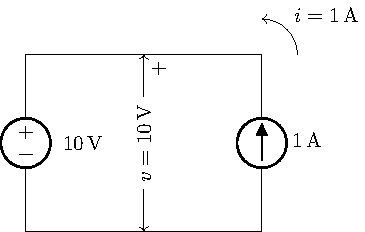
\includegraphics[height = 4cm, keepaspectratio = true]{connected_sources}
    \caption{Example of a connected voltage and current source.}
\end{figure}
\begin{itemize}
    \item The voltage source sets $v$ to \SI{10}{\volt}, with the upper wire being positive.
    \item The current source sets $i$ to \SI{1}{\ampere}, flowing anticlockwise.
    \item Therefore \SI{10}{\watt} of power is produced by the current source and dissipated by the voltage source.
\end{itemize}
\begin{enumerate}
    \item Two voltage sources must be connected at the same terminals and supply the same voltage.
    \item Two current sources must flow in the same direction and supply the same current.
\end{enumerate}
\subsection{Invalid Circuits}
\begin{figure}[H]
    \centering
    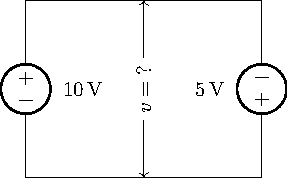
\includegraphics[height = 4cm, keepaspectratio = true]{invalid_voltage_sources}
    \caption{Voltage terminals are incorrect, and voltages are different.}
\end{figure}
\begin{figure}[H]
    \centering
    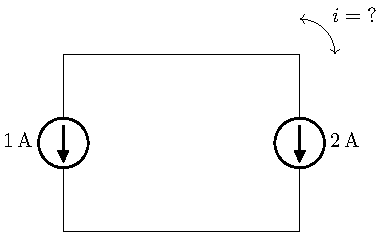
\includegraphics[height = 4cm, keepaspectratio = true]{invalid_current_sources}
    \caption{Current flows oppose each other, and currents are different.}
\end{figure}
\subsection{Resistors}
\begin{definition}[Resistor]
    Resistors dissipate power, and the voltage across both terminals is proportional to the current.
\end{definition}
\begin{figure}[H]
    \centering
    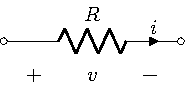
\includegraphics[height = 4cm, keepaspectratio = true]{resistor}
    \caption{}
\end{figure}
\begin{theorem}[Voltage through a resistor]
    \begin{equation*}
        v=iR
    \end{equation*}
    \begin{equation*}
        R=\frac{\rho L}{A}
    \end{equation*}
\end{theorem}
\newpage
\section{Simple Resistive Circuits}
\subsection{Ignored Physics}
\begin{enumerate}
    \item Electrical effects occur instantaneously, so there is no time delay along the wires.
    \item The net charge on every component is zero. Charge is never lost or gained.
    \item There is no magnetic coupling between the components.
\end{enumerate}
\subsection{Kirchhoff's Laws}
\begin{definition}[Kirchhoff's Current Law (KCL)]
    The sum of all currents into a node equals zero.
    \begin{equation*}
        \sum i_{node} = 0
    \end{equation*}
\end{definition}
\begin{definition}[Kirchhoff's Voltage Law (KVL)]
    The sum of all voltages around a loop equals zero.
    \begin{equation*}
        \sum v_{loop} = 0
    \end{equation*}
\end{definition}
\subsection{Series and Parallel Circuits}
\begin{definition}
    Elements connected end-to-end are in series. If both ends of an element are connected directly to another element, the two elements are in parallel.
\end{definition}
\begin{table}[H]
    \centering
    \begin{tabular}{c | c c}
        \toprule
        \textbf{Element} &  \textbf{Series} & \textbf{Parallel} \\
        \midrule
        Current Source & $\displaystyle i_{eq} = i_1 = i_2 = \cdots = i_n$             & $i_{eq} = \displaystyle \sum_k i_k$ \\
        Voltage Source & $\displaystyle v_{eq} = \sum_{k=1}^n v_k$                     & $\displaystyle v_{eq} = v_1 = v_2 = \cdots = v_n$ \\
        Resistor       & $\displaystyle R_{eq} = \sum_{k=1}^n R_k$                     & $\displaystyle \frac{1}{R_{eq}} = \sum_{k=1}^n \frac{1}{R_k}$ \\
        Inductor       & $\displaystyle L_{eq} = \sum_{k=1}^n L_k$                     & $\displaystyle \frac{1}{L_{eq}} = \sum_{k=1}^n \frac{1}{L_k}$ \\
        Conductor      & $\displaystyle \frac{1}{C_{eq}} = \sum_{k=1}^n \frac{1}{C_k}$ & $\displaystyle C_{eq} = \sum_{k=1}^n C_k$ \\
        \bottomrule
    \end{tabular}
    \caption{Equivalent values for various components connected in series and parallel.}
    % \label{}
\end{table}
These equations can be used to simplify a complex circuit.
\begin{proof}
    Using KVL for voltage sources connected in series
    \begin{align*}
        v_1 + v_2 + \cdots + v_n - iR &= 0 \\
        v_1 + v_2 + \cdots + v_n &= iR
    \end{align*}
    Let $v_{eq}$ be the voltage across the resistor so that
    \begin{equation*}
        v_{eq} = iR
    \end{equation*}
    Therefore
    \begin{equation*}
        v_{eq} = v_1 + v_2 + \cdots + v_n
    \end{equation*}
    
    As the current through resistors in series remains the same, using KVL we have
    \begin{align*}
        v - iR_1 - iR_2 - \cdots - iR_n &= 0 \\
        v &= i\left(R_1 + R_2 + \cdots + R_n\right) \\
        v &= iR_{eq}
    \end{align*}
    Hence the resistance across multiple resistors in series is equivalent to the sum of the resistances.
\end{proof}
\subsection{Voltage and Current Dividers}
\begin{definition}[Voltage Divider]
    A voltage divider is a circuit that divides a voltage in the proportion of the series resistances.
\end{definition}
\begin{figure}[H]
    \centering
    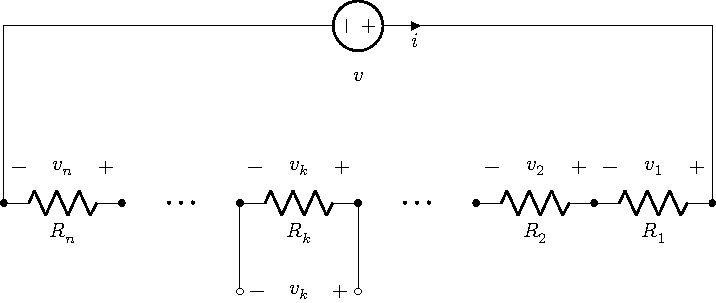
\includegraphics[height = 4cm, keepaspectratio = true]{voltage_divider}
    \caption{Resistors connected in series to a voltage source.}
    % \label{}
\end{figure}
\begin{theorem}
    \begin{equation*}
        v_k = v \frac{R_k}{R_{eq}}
    \end{equation*}
\end{theorem}
\begin{proof}
    The current through any resistor is
    \begin{equation*}
        i = \frac{v}{R_{eq}}
    \end{equation*}
    Therefore the voltage drop in any resistor is
    \begin{align*}
        v_k &= i R_k \\
        v_k &= \frac{v}{R_{eq}} R_k
    \end{align*}
\end{proof}
\begin{definition}[Current Divider]
    A voltage divider is a circuit that divides a voltage in the proportion of the series resistances.
\end{definition}
\begin{theorem}
    \begin{equation*}
        i_k = i \frac{R_{eq}}{R_k}
    \end{equation*}
\end{theorem}
\newpage 
\section{Diodes}
\newpage
\section{Mesh Analysis}
\newpage
\section{Source Transformation}
\newpage
\section{Inductors and Capacitors}
\newpage
\section{RC and RL Circuits}
\newpage
\section{Operational Amplifiers}
\newpage
\section{Sinusoidal Signals}
\newpage
\section{Frequency Response}
\newpage
\section{Filters and Rectifiers}
\newpage
\section{Zener Diodes and Voltage Regulators}
\newpage

\end{document}